\section{Object reconstruction and selection}
\label{sec:object_reconstruction}

The reconstruction and selection of physics objects, i.e.\ objects
representing the signature of particles produced in the
$pp$-collision, is described in the following. The most relevant
objects in this search are electrons, muons, \tauhadvis, jets,
$b$-tagged jets, and the missing transverse momentum. These objects
are reconstructed and identified using different algorithms targeting
their distinct signature in the ATLAS detector. The same algorithms
are used to reconstruct and identify objects in simulation and in data
recorded with the detector.  Differences between the performance of
the reconstruction and selection in simulation and data are accounted
for by dedicated calibration measurements of efficiencies, energy /
momentum scales and resolutions. Uncertainties on these measurements
are propagated to the final results by performing variations of these
properties in simulation.

The following introduces the reconstruction and selection of physics
objects relevant to this analysis. A discussion of objects not
directly used in this analysis is omitted.



% The trajectories of charged particles...

Charged particle tracks are reconstructed from their signature in the
inner tracking detectors of the ATLAS detector. They are a fundamental
input to other reconstruction and identification algorithms where they
are used at different levels of reconstruction quality.

The baseline selection for charged particle tracks requires
$\pT > \SI{500}{\MeV}$ and $|\eta| < \num{2.5}$ in addition to several
requirements on the number of hits, the number of missing hits
(holes), and the number of hits shared between multiple tracks in the
silicon-based tracking detectors.

And impact parameter requirements.

\cite{PERF-2015-08}

Tracks measured in the inner detector are used to determine the $pp$
interaction vertices, which are the points in the ATLAS detector where
a scatter interaction between protons took place. For a given event
recorded by the detector, the vertex with the largest sum of $\pT^2$
of associated tracks and at least two associated tracks with
$\pT > \SI{500}{\MeV}$ is considered as the primary vertex of the
event. Other vertices with at least two tracks are considered as
vertices originating from pile-up~\cite{PERF-2015-01}.

The selection of objects directly used in this search is described in
the following. More restrictive selections on these objects will be
applied as part of the signal region event selection.
\begin{description}

\item[Electrons] are required to have $\pT > \SI{7}{\GeV}$ and to be
  reconstructed within the acceptance of the tracking detectors
  $|\eta| < \num{2.47}$. Electrons in the transition region between
  the barrel and end-cap electromagnetic calorimeters of the ATLAS
  detector, $1.37 < |\eta| < 1.52$, are rejected. A likelihood-based
  discriminant is used for electron identification to reject electron
  candidates originating from jets and non-prompt electrons (e.g.\
  from photon conversions or decays of hadrons) by exploiting
  variables sensitive to the shower-shape, track quality, information
  about transition radiation emission in the TRT, and spatial and
  momentum matching between track and calorimeter
  cluster~\cite{EGAM-2018-01}. The loose electron identification
  working point is used corresponding to an average identification
  efficiency of about \SI{93}{\percent}~\cite{EGAM-2018-01}.

  % FCLoose
  % topoetcone20/pT < 0.2
  % ptvarcone20_TightTTVA_pt1000/pT < 0.15
  Electron candidates with high activity in the vicinity of the
  electron are rejected by making a loose requirement on both
  calorimeter- and track-based isolation variables
  ($E_{\text{T}}^\text{cone20} / \pT < 0.2$ and
  $p_{\text{T}}^{\text{varcone20}}/ \pT < 0.15$ as described in
  Ref.~\cite{EGAM-2018-01}). The electron selection efficiency of the
  isolation requirement exceeds \SI{95}{\percent} for electrons with
  $\pT > \SI{20}{\GeV}$, quickly approaching efficiencies close to
  \SI{100}{\percent} at larger transverse
  momenta~\cite{EGAM-2018-01}. This requirement is inverted as part of
  the \faketauhadvis background estimation in the \lephad channel to
  provide a control region enhanced in multi-jet events.

  % Energy calibration???

  % Post-selection:
  % Medium LH
  % pT > 18 GeV

\item[Muons] are required to have $\pT > \SI{7}{\GeV}$ and pass the
  loose identification working point. Muons passing the loose working
  point are a superset of medium muons which are defined according to
  Ref.~\cite{MUON-2018-03} as: muons passing either the
  \emph{combined} or \emph{inside-out combined} reconstruction in
  $|\eta| < 2.5$; muons passing either the \emph{muon-spectrometer
    extrapolated} or \emph{silicon-associated forward} reconstruction
  in $2.5 < |\eta| < 2.7$. Various requirements are set on the muon
  reconstruction quality and matching between ID and MS tracks which
  depend on the muon reconstruction type and detector region. The
  loose identification working point additionally allows for
  \emph{calorimeter-tagged} and \emph{segment-tagged} muons in
  $|\eta| < 0.1$, a region insufficiently covered by the MS, to
  improve the muon selection efficiency.

  Muons are required to pass a loose isolation working point based on
  an isolation requirement combining information on charged and
  neutral particle signatures using a particle flow approach
  ($p_{\text{T}}^{\text{varcone30}} + 0.4 \times
  E_{\text{T}}^{\text{neflow20}} < 0.16$~\cite{MUON-2018-03}). The
  isolation requirement is inverted to provide a control region for
  the \faketauhadvis estimation in the \lephad channel.

  % What happens with muons for the muon in jet correction?

  % isPflowLoose_VarRadIso
  % (ptvarcone30_TightTTVA_pt500 + 0.4 neflowisol20) / pT < 0.16

  % Post-selection
  % pT > 17 GeV
  % Medium muon + |\eta| < 2.5
  % Iso???

\item[\tauhadvis] are required to have $\pT > \SI{20}{\GeV}$ and
  $|\eta| < 2.5$, rejecting candidates reconstructed in the transition
  region between barrel and end-caps ($1.37 < |\eta| < 1.52$).

  Candidate \tauhadvis are required to have either 1 or 3 charged
  particle tracks identified according to a multivariate track
  classification algorithm as originating from a charged pion produced
  in the \taulepton decay. The combined electric charge of these
  tracks is required to be $\pm 1\,e$.

  A BDT-based electron veto algorithm is applied to 1-prong \tauhadvis
  candidates to reject candidates originating from the signature of an
  electron in the detector. The algorithm is \SI{95}{\percent}
  efficient in selecting \tauhadvis candidates matched to \tauhad
  decays.

  A loose \tauhadvis identification using the RNN algorithm
  (cf.~\Cref{sec:tauid}) that combines the information of high-level
  variables, with sequences of charged particle tracks and clusters
  that are associated to the \tauhadvis candidates. This working point
  is defined to yield a true \tauhadvis selection efficiency of
  \SI{85}{\percent} (\SI{75}{\percent}) in simulated
  $\gamma^* \to \tauhad\tauhad$ events for 1-prong (3-prong)
  \tauhadvis. The mean \faketauhadvis selection
  efficiency\footnote{The \faketauhadvis selection efficiency depends
    strongly on the transverse momentum of \tauhadvis candidates thus
    only a mean value is given.} of the loose working point is about
  \SI{5}{\percent} (\SI{1}{\percent}) for 1-prong (3-prong) \tauhadvis
  candidates from simulated multi-jet
  events~\cite{ATL-PHYS-PUB-2019-033}.

  The \tauhadvis energy calibration is performed by combining a
  calorimeter-based energy measurement with information from the tau
  particle flow algorithm~\cite{PERF-2014-06} in boosted regression
  trees.

  % \todo[inline]{taus: seeding; energy scale (LC \& BRT); track selection;
  %   acceptance; Tau-ID (jet \& e)}

\item[Anti-\tauhadvis] adhere to the same selection criteria as
  \tauhadvis except for the \tauhadvis identification requirement
  which is partially inverted. \tauhadvis candidates are considered to
  be anti-\tauhadvis if they do not pass the loose \tauhadvis
  identification working point but exceed a very loose selection on
  the \tauhadvis identification score of $\text{RNN score} > 0.01$,
  which corresponds to a true \tauhadvis selection efficiency of about
  \SI{99}{\percent} in simulated $\gamma^* \to \tauhad\tauhad$.

  Anti-\tauhadvis are only considered when events have fewer than two
  (one) \tauhadvis passing the selection criteria of the \hadhad
  (\lephad) channel. In this case, anti-\tauhadvis are randomly
  selected until the required number of (anti-)\tauhadvis candidates,
  two in the \hadhad and one in the \lephad channel, is
  achieved. Anti-\tauhadvis that are not selected by the random
  anti-\tauhadvis selection are treated as jets and will later be
  removed as part of the overlap removal procedure.

  All search channels use the presence of a selected anti-\tauhadvis
  to define control regions used to derive data-driven estimates of
  backgrounds containing \faketauhadvis using the fake factor method.

\item[Jets] are reconstructed using the anti-\kt
  algorithm~\cite{Cacciari:2008gp} with a radius parameter
  of~$R = 0.4$. The inputs to the jet algorithm are provided by a
  particle flow reconstruction algorithm, described in
  Refs.~\cite{PERF-2015-09,JETM-2018-05}, exploiting the superior
  momentum resolution of the tracking system for charged particles
  with low transverse momenta by replacing the calorimetric
  measurement of their energy with a tracking-based momentum
  measurement, necessitating the subtraction of energy deposits by
  charged particles in the calorimeter. The particle flow algorithm
  provides an improved jet energy and angular resolution as well as
  pile-up stability compared to jets constructed based on topological
  clusters in the calorimeters (at EM scale)
  only~\cite{PERF-2015-09,JETM-2018-05}.

  Jets in the central region defined by $|\eta| < 2.5$ are required to
  fulfil $\pT > \SI{20}{\GeV}$; jets in the forward regions defined
  by $2.5 < |\eta| < 4.5$ are required to fulfil
  $\pT > \SI{30}{\GeV}$. Jets originating from pile-up are suppressed
  by ensuring that jets pass jet-vertex-tagger (JVT)
  requirements. Jets in the central region are required to pass the
  tight working point of the JVT~\cite{PERF-2014-03}. Jets in the
  forward region, which lack tracking system coverage, are required to
  fulfil the loose working point of a dedicated jet-vertex-tagger for
  forward jets~\cite{PERF-2016-06-witherratum,ATL-PHYS-PUB-2019-026}.

  A multivariate $b$-tagging algorithm is applied to all jets in the
  central region to identify jets originating from $b$-quarks,
  distinguishing them from jets initiated by gluons or quarks of
  light- or charm-flavour. The \textsc{DL1r}
  algorithm~\cite{FTAG-2018-01,ATL-PHYS-PUB-2017-013} is used which
  combines the scores of several low-level taggers that exploit the
  signature of displaced decays of $b$-hadrons using information on
  the track impact parameters (\textsc{IP2D}, \textsc{IP3D} \&
  \textsc{RNNIP}) and secondary vertices (\textsc{SV1} \&
  \textsc{JetFitter}). A $b$-tagging working point with an efficiency
  of \SI{77}{\percent} of correctly tagging $b$-jets in \ttbar is
  used.

\item[Missing transverse momentum (\pTmiss)] is used to reconstruct
  the total transverse momentum of (undetected) weakly-interacting
  particles produced in the hard interaction. In this search it is
  used to reconstruct the signatures of neutrinos produced in decays
  of \tauleptons and semi-leptonic decays of hadrons.

  An object-based definition of the missing transverse
  momentum~\cite{PERF-2016-07} is adopted that uses reconstructed and
  calibrated objects, i.e.\ electrons, muons, \tauhadvis, and jets as
  defined previously after an ambiguity resolution step introduced
  in~\Cref{sec:overlap_removal}, as inputs to the \pTmiss
  reconstruction. Soft charged particle radiation that is not part of
  any reconstructed object is accounted for by the so-called track
  soft term. The track soft term is defined as the vectorial sum of
  charged particle track $\myvec{\pT}$ over all tracks passing track
  quality criteria that are associated to the primary vertex of the
  hard interaction but not any reconstructed object. The object-based
  \pTmiss is subsequently reconstructed as the negative vectorial sum
  of transverse momenta of calibrated objects and the track soft term.

  The vector of the missing transverse momentum in the transverse
  plane is denoted as \pTmiss and its magnitude as \pTmissAbs,
  hereafter.
\end{description}


\subsection{Overlap Removal}
\label{sec:overlap_removal}

The reconstruction and selection of physics objects described
previously does not ensure that any detector signature can be
unambiguously assigned to exactly one reconstructed object. This
ambiguity is resolved by performing an overlap removal procedure which
rejects objects that can be associated, either geometrically or by
shared charged particle tracks, with an object of higher priority. In
the case of geometric matching the association is performed on the
basis of the angular distance
\begin{align*}
  \dRy = \sqrt{\Delta y^2 + \Delta \phi^2} \,\text{,}
\end{align*}
where $\Delta y$ and $\Delta \phi$ refers to the differences in
rapidity and polar angle of two objects, respectively.

A sequential procedure is used to resolve the overlaps of
reconstructed physics objects. The procedure is summarised
in~\Cref{tab:overlap_removal} following recommendations developed by
the ATLAS collaboration. Two additional steps are added to resolve
overlaps between jets and anti-\tauhadvis which aim to improve the
signal selection efficiency in this search.

\begin{table}[htbp]
  \centering

  % https://gitlab.cern.ch/atlas/athena/tree/21.2/PhysicsAnalysis/AnalysisCommon/AssociationUtils/
  % Harmonization note: https://cds.cern.ch/record/1743654/files/ATL-COM-PHYS-2014-451.pdf

  \caption{Summary of the sequential overlap removal algorithm with
    rows representing steps of the procedure. Steps are executed from
    top to bottom, rejecting objects in the \emph{Reject} column in
    favour of objects in the \emph{Accept} column if the condition is
    fulfilled. The last three steps }%
  \label{tab:overlap_removal}

  \resizebox{\textwidth}{!}{%
    \begin{tabular}{lll}
  \toprule
  Reject & Accept & Condition \\
  \midrule

  % https://gitlab.cern.ch/atlas/athena/-/blob/21.2/PhysicsAnalysis/AnalysisCommon/AssociationUtils/Root/EleEleOverlapTool.cxx
  $e_1$ & $e_2$ & $e_1$ and $e_2$ share the charged particle track and $\pT(e_1) < \pT(e_2)$. \\[0.5em]

  % https://gitlab.cern.ch/atlas/athena/-/blob/21.2/PhysicsAnalysis/AnalysisCommon/AssociationUtils/Root/TauLooseEleOverlapTool.cxx
  \tauhadvis & $e$ & $\dRy < 0.2$ and $e$ passes the loose likelihood-based electron identification. \\[0.5em]

  % https://gitlab.cern.ch/atlas/athena/-/blob/21.2/PhysicsAnalysis/AnalysisCommon/AssociationUtils/Root/TauLooseMuOverlapTool.cxx
  \tauhadvis & $\mu$ & $\dRy < 0.2$ and either: \\
         && \hspace{0.5em}-\, \tauhadvis $\pT \leq \SI{50}{\GeV}$: $\pT(\mu) > \SI{2}{\GeV}$ \\
         && \hspace{0.5em}-\, \tauhadvis $\pT > \SI{50}{\GeV}$: $\pT(\mu) > \SI{2}{\GeV}$ and $\mu$ passes combined muon reconstruction. \\[0.5em]

  % https://gitlab.cern.ch/atlas/athena/-/blob/21.2/PhysicsAnalysis/AnalysisCommon/AssociationUtils/Root/EleMuSharedTrkOverlapTool.cxx
  $\mu$ & $e$ & $\mu$ is calorimeter-tagged and shares inner detector track with $e$. \\[0.5em]
  $e$   & $\mu$ & Both share the inner detector track. \\[0.5em]

  % Note: We do not use heavy flavour aware OLR

  % https://gitlab.cern.ch/atlas/athena/-/blob/21.2/PhysicsAnalysis/AnalysisCommon/AssociationUtils/Root/EleJetOverlapTool.cxx
  jet   & $e$ & $\dRy < 0.2$ \\[0.5em]
  $e$   & jet & $\dRy < 0.4$ \\[0.5em]

  % https://gitlab.cern.ch/atlas/athena/-/blob/21.2/PhysicsAnalysis/AnalysisCommon/AssociationUtils/Root/MuJetOverlapTool.cxx
  jet   & $\mu$ & The ID track of the muon is ghost-associated$^\dagger$ to the jet and the jet has fewer than three \\
         && ghost-associated ID tracks with $\pT > \SI{500}{\MeV}$. \\[0.5em]
         % && \hspace{0.5em}-\, The jet has fewer than three ghost-associated ID tracks with $\pT > \SI{500}{\MeV}$ \\
         % && \hspace{0.5em}-\, $\pT(\mu) / \pT(\text{jet}) > 0.5$ and $\pT(\mu) / \sum \pT(\text{track}) > 0.7$, where the sum goes over \\

  $\mu$ & jet & $\dRy < 0.4$ \\

  %jet - 𝜇: Reject jet if 𝑁track < 3 (𝑝 T, track > 500 MeV), and Δ𝑅 𝑦 < 0.2

  \midrule
  jet & \tauhadvis & ... \\[0.5em]
  anti-\tauhadvis & jet & ... \\[0.5em]
  jet & anti-\tauhadvis & ... \\
  \bottomrule
\end{tabular}

%%% Local Variables:
%%% mode: latex
%%% TeX-master: "../phd_thesis"
%%% End:

  }
\end{table}

The overlap removal establishes the following priority between jets,
\tauhadvis, and selected anti-\tauhadvis:
\begin{center}
  \tauhadvis > \btagged jet > anti-\tauhadvis > un-tagged jet.
\end{center}
An alternative prioritisation given by
\begin{center}
  \btagged jet > \tauhadvis > anti-\tauhadvis > un-tagged jet
\end{center}
is also investigated but found to reduce the signal acceptance when
selecting events with 2 \btagged jets due to the limited \tauhadvis
rejection of the \textsc{DL1r} \btag algorithm at the
\SI{77}{\percent} efficiency working point. The alternative leads to a
relative reduction in SM \HH signal acceptance by \SI{8}{\percent}
(\SI{13}{\percent}) in the \lephad (\hadhad) channels. Thus \tauhadvis
take precedence over $b$-tagged jets in the overlap removal procedure,
maximising the signal acceptance.

% Due to a bug in the PFlow jet reconstruction, an additional OLR step removing
% prompt muons being reconstructed as fake jets is implemented in the official ASG
% OLR tool.

\todo[inline]{Truth labelling of jets in simulation cf.\ VHbb evidence paper}
\todo[inline]{Truth labelling of fake taus in simulation}

\subsection{$H \to \bbbar$ candidate reconstruction and momentum
  corrections for $b$-tagged jets}%
\label{sec:hbb_reco}%
\label{sec:bjet_momentum_corrections}

\todo{Move to event selection???}

The Higgs boson candidate decaying into a pair of $b$-quarks is
reconstructed using jets in the central region of the detector
($|\eta| < 2.5$). In regions requiring two $b$-tagged jets, the
four-momentum of the Higgs boson candidate is reconstructed by summing
the four-momenta of both $b$-tagged jets. The Higgs boson candidate
four-momentum in regions with fewer than two $b$-tagged jets, which
are used as control and validation regions, is reconstructed from the
sum of four momenta of either the $b$-tagged jet and the \pT-leading
un-tagged jet (1 $b$-tag regions) or the sum of the two \pT-leading
un-tagged jets (0 $b$-tag regions). Regions with more than two
$b$-tagged jets are not considered in this search. The reconstructed
Higgs boson candidate is used to calculate the invariant mass of the
$\bbbar$-system, \mBB, which is an important variable to distinguish
signals from backgrounds.

Corrections are applied to $b$-tagged jets in order to improve the
scale and resolution of the $b$-jet momentum reconstruction,
consequently improving the scale and resolution of the reconstructed
\mBB and thus its discrimination power between signals and
backgrounds.

The $b$-jet momentum corrections are applied in addition to the
standard jet calibration~\cite{JETM-2018-05}, targeting the effects of
out-of-cone radiation and semi-muonic $b$- or $c$-hadron decays inside
of the $b$-jet on the reconstructed jet four-momentum. Two separate
corrections, which were previously used by the ATLAS collaboration in
Refs.~\cite{HIGG-2016-29,HIGG-2018-04,HIGG-2018-51}, are applied:
\begin{description}

\item[Muon-in-jet correction] Muons produced in decays of $b$- or
  $c$-hadrons in $b$-jets deposit little energy in the calorimeters
  leading to an underestimation of the jet four-momentum. The
  muon-in-jet correction is applied when a muon with
  $\pT > \SI{4}{\GeV}$ passing the \emph{medium} selection working
  point can be found within a variable size cone (shrinking with
  increasing \pT of the muon) centred on the jet axis. No
  requirements on the isolation of muons for the muon-in-jet
  corrections are made. In case one or more muons fulfilling the
  criteria are selected, the four-momentum of the muon closest to the
  jet axis, after correcting for the energy it deposited in the
  calorimeters, is added to the four-momentum of the jet.

\item[\pTreco correction] The \pTreco correction aims to correct for
  out-of-cone radiation as well as momentum carried away by neutrinos
  produced in semi-muonic decays of hadrons in the jet. It is derived
  from $b$-tagged jets in simulated \ttbar events as a function of the
  \pT of the reconstructed jets, \pTreco, and separately for jets
  containing a muon and jets that do not contain a muon following the
  approach used for the muon-in-jet correction. The correction is
  applied as a multiplicative factor on the jet momentum scale and is
  derived as the ratio $p_{\text{T}}^{\text{truth}} / \pTreco$ in bins
  of \pTreco, where $p_{\text{T}}^{\text{truth}}$ is the transverse
  momentum of the truth jet, a jet constructed from generator-level
  particles, that is geometrically matched to the jet at
  reconstruction-level.

\end{description}
Both corrections are performed at the level of individual jets and do
not explicitly include information about the remainder of the event.

The effect of the corrections on the reconstructed \mBB for simulated
SM \HH events produced via \ggF in the \hadhad channel is depicted
in~\Cref{fig:bjet_momentum_corr_mbb}. The improvement in the $b$-jet
momentum scale and resolution from the muon-in-jet correction and the
\pTreco correction lead to a relative reduction of the width of the
Higgs boson mass peak in \mBB of about \SI{13}{\percent}, as measured
by the full width at half maximum.

\begin{figure}[htbp]
  \centering

  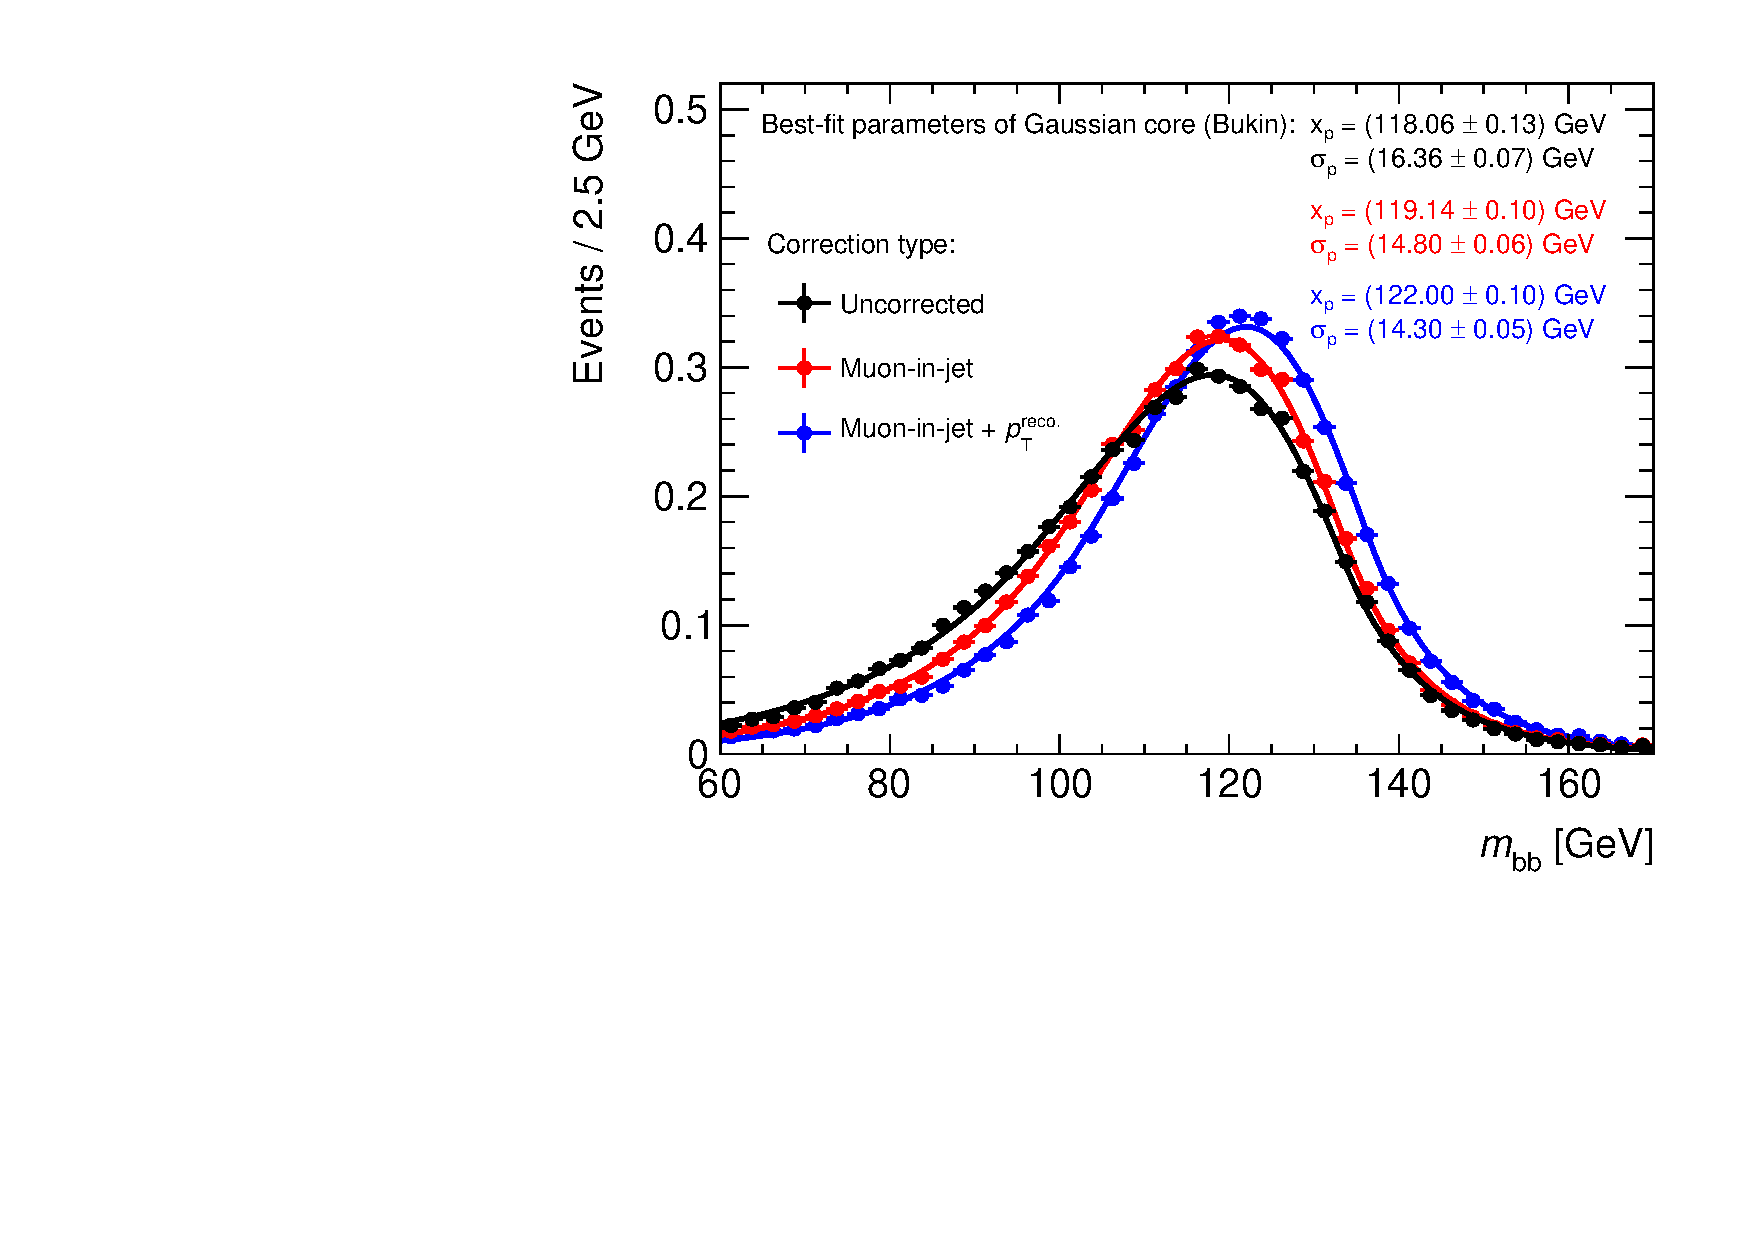
\includegraphics[width=0.65\textwidth]{reconstruction/bjet_corrections}

  \caption{Effects of different $b$-jet momentum corrections on the
    reconstructed \mBB of $H \to \bbbar$ candidates from simulated SM
    \HH events in the \hadhad channel. Bukin
    functions~\cite{Bukin:2007zha}\todo[inline]{Check me} are fitted
    to binned distributions obtained from simulation. The location of
    the peak maximum is given by $x_{\text{p}}$ and the full width at
    half maximum divided by $2\sqrt{2 \ln 2}$ is given by
    $\sigma_{\text{p}}$ (yielding width scales comparable to the
    standard deviation of a Normal distribution). The uncorrected
    distribution is obtained using the standard jet calibration
    without further corrections for $b$-jets.}%
  \label{fig:bjet_momentum_corr_mbb}
\end{figure}


\subsection{$H \to \tau^{+}\tau^{-}$ candidate reconstruction}%
\label{sec:htautau_reco}

\todo{Move to event selection???}

Reconstruction of the $H \to \tau^{+}\tau^{-}$ candidate's
four-momentum in signal events is challenging due to the presence of
at least two neutrinos originating from decays of \tauleptons that
cannot be measured directly. The starting point of the reconstruction
are the visible decay products from \taulepton decays. In the \hadhad
channel these are given by the two \tauhadvis candidates, while in the
\lephad channel the visible decay products are the \tauhadvis
candidate and either an electron or a muon. To obtain the
four-momentum of the di-$\tau$ system, %
% consisting of visible and invisible decay products
additional information on the neutrinos produced from the \taulepton
decay is required. The allowed configurations of neutrinos from
\taulepton decays can be restricted using the observed visible decay
products and kinematic constraints from the known mass of the
\taulepton and the measurement of \pTmiss under the assumption that
its sole source are neutrinos produced from decays of
\tauleptons. However, the resulting system of kinematic equations is
underdetermined leaving multiple degrees of freedom for the unobserved
neutrinos.

The Missing Mass Calculator (MMC) technique~\cite{Elagin:2010aw} is
used to estimate the four-momentum of the di-$\tau$ system and thus
its invariant mass, referred to as \mMMC hereafter. The MMC uses the
fact that not all configurations of neutrinos are equally likely,
assigning a probability density for every configuration conditional on
the \taulepton decay mode and other properties of the visible decay
products. In addition, the constraint on the total neutrino transverse
momentum from the \pTmiss measurement are relaxed to allow for
measurement errors within the experimental resolution, the resolution
being parameterised as a function of the event activity\footnote{The
  event activity, also referred to as $\sum \ET$, is the scalar sum
  of transverse momenta of all hard objects produced in an event and
  the track soft term.} and jet multiplicity. The probability density
functions used by the MMC are derived from simulation of resonant
production of \taulepton pairs.

For any single event the MMC estimates the conditional
distribution\footnote{The distribution is conditional on the observed
  properties of the event such as the reconstructed four-momenta of
  the visible \taulepton decay products, the \taulepton decay mode,
  \pTmiss, $\sum \ET$, and the jet multiplicity.} of an observable of
interest depending on unobserved neutrino properties, for example the
mass of the di-$\tau$ system, using simulation. %
% The distribution of an observable of interest that depends on
% unobserved neutrino properties given, for example the mass of the
% di-$\tau$ system, can be estimated using simulation.
A sequence of kinematically allowed neutrino configurations is
generated using Markov Chain Monte Carlo according to the
(conditional) probability density that describes the distribution of
neutrino configurations. For every configuration the value of the
observable of interest is calculated and filled into a histogram,
which serves as a binned approximation of the observable's conditional
distribution. Finally, the most probable value of the observable is
used as an event-level estimator.

Frequently, the most probable di-$\tau$ invariant mass is used as the
estimator when the mass is of primary interest such as in measurements
of $H \to \tau^{+}\tau^{-}$~\cite{HIGG-2019-09}. However, in searches
for Higgs boson pair production it is desirable to estimate the entire
four-momentum of the di-$\tau$ system as it allows to calculate the
invariant mass of the $HH$-system, \mHH, when combined with the
four-momentum of the $H \to \bbbar$ candidate. Instead of the most
probable mass estimator, an estimator based on the most probable
neutrino momenta is used, allowing to reconstruct the four-vector of
the di-$\tau$ system.

A description of the technical implementation of the MMC used by the
ATLAS collaboration is given in Ref.~\cite{huebner} which is used as
the basis for the four-momentum reconstruction of the
$H \to \tau^{+}\tau^{-}$ candidate in this search.

%%% Local Variables:
%%% mode: latex
%%% TeX-master: "../../phd_thesis"
%%% End:
